\section{Empirical Evaluation}
%- resultados basicos segun los distintos encodings
%- resultados comparativos de cuando empiezan a fallar en mapas cuadrados vacios
%- analisis varios (porq el encoding mejora o empeora)
%- hablar de cosas negativas
%- empezar a ver una cota tentativa segun numero de celdas.

%- comparar cambiar restricciones del dijkstra. Un problema en grilla cuadrada.
%- usar la version mas simple.


We compared our algorithm to publicly available search-based solvers as well as MDD-SAT \cite{Surynek14} (enc=mdd), on congested grids. We ran two state-of-the-art search algorithms:  EPEA* \cite{Goldenberg14}, and ICBS-h \cite{FelnerLB00KK18}.

The code used for our implementation was written in Python 3.7 using Clingo 5.3 () for the ASP solver. Clingo was run with 4 threads in \textit{parallel-mode}, and using \textit{usc} as the optimization strategy. The search based algorithms use a implementation written C\#, based on the implementation in \cite{FelnerLB00KK18}. The MDD-SAT algorithm use a implementation written C++ based in (cita de surynek)

All the experiments were tested on a 3.40GHz Intel Core i5-3570K computer with 8GB of memory. We set a runtime limit of 5 minutes for all the problems.

\subsection{Open $N$ x $N$ grids experiments} First, we experimented on different empty grids (No obstacles), with sizes $N=\{8,16,32,64\}$. For each one of these grids we generated $10$ instances
for each number of agents between $A=\{2,4, \ldots N^2 -2 \}$. All the agents initial positions and goals were randomly placed. We compared different encodings, where ASP-basic is a basic encoding that uses quadratic conflict resolution and grid dependent penalties. ASP-indep uses quadratic conflict resolution and grid independent penalties. Finally, ASP-lin-indep uses linear conflict resolution and grid independent penalties.


In figure we show the \emph{breaking point}. of the thingy


\subsection{N x N grids with random obstacles experiments} 
Next, we experimented on $8\times 8$ and $20\times 20$ randomly generated problems with 10\% obstacles. For $8\times8$ (resp.~$20\times 20$) we generate 150 (resp.~160) problems with the number of agents in $\{4,\dots,18\}$ (resp.~$\{20,22,\ldots,50\}$). Success rates, and number of problems solved versus time are shown in Figure ~\ref{fig_obs}. 

In the $8\times8$  tests all of our encodings outperform the other algorithms in terms of success rate, this shows the benefits of using ASP as a solving mechanism. On the other hand, seeing the results on the curves of the solving time shows that there's an important factor on the basic time needed to solve. Esto se explica debido al proceso de grounding que se debe hacer al inicio de cada instanciación.

En el caso de las grillas de $20x20$, podemos apreciar como la linearización de las reglas para conflictos toman una gran importancia, logrando resolver prácticamente todos los problemas. Por otro lado nuestras codificaciones básicas que usan las reglas básicas para conflictos empiezan a fallar rápidamente con más agentes, esto debido a que el número de constraints es cuadrático con respecto al número de agentes. Es interesante destacar que el uso de grid-independent encoding no resulta en cambios importantes en estas grillas.

Otro punto importante es el uso del método de USC con respecto a BB. USC parte con una solución costo mínimo que no necesariamente satisface los constraints, luego hace cambios hasta encontrar una solución que cumpla estos constraints. bb por otro lado primero encuentra una solución que satisface lo constraints y hace cambios a la solución hasta encontrar y demostrar una solución de costo mínimo. Debido a que normalmente la solución a los problemas en MAPF es más cercana a la solución óptima ignorando los conflictos es que USC muestra mejores resultados.

\subsection{Warehouse experiments}
Also, we experimented on a the warehouse grid shown in Figure ~\ref{fig_ware}. La elección de las posiciones iniciales y objetivos de los agentes es de manera aleatoria sobre las dos columnas libres en cada borde de la grilla. We generated $10$ instances for each number of agents between $a=\{4, \ldots, 16\}$.

Estos resultados muestran los grandes beneficios de nuestro encoding en grillas con muchos conflictos posibles. En este mapa  hay pocos espacios libres, en particular debido a que $|V|$ es mucho más pequeño nuestra codificación es más compacta. Por otro lado, estos resultados muestran que en problemas en que el número de conflictos posibles es alto nuestro algoritmo no se muestra afectado.



\begin{figure*}
    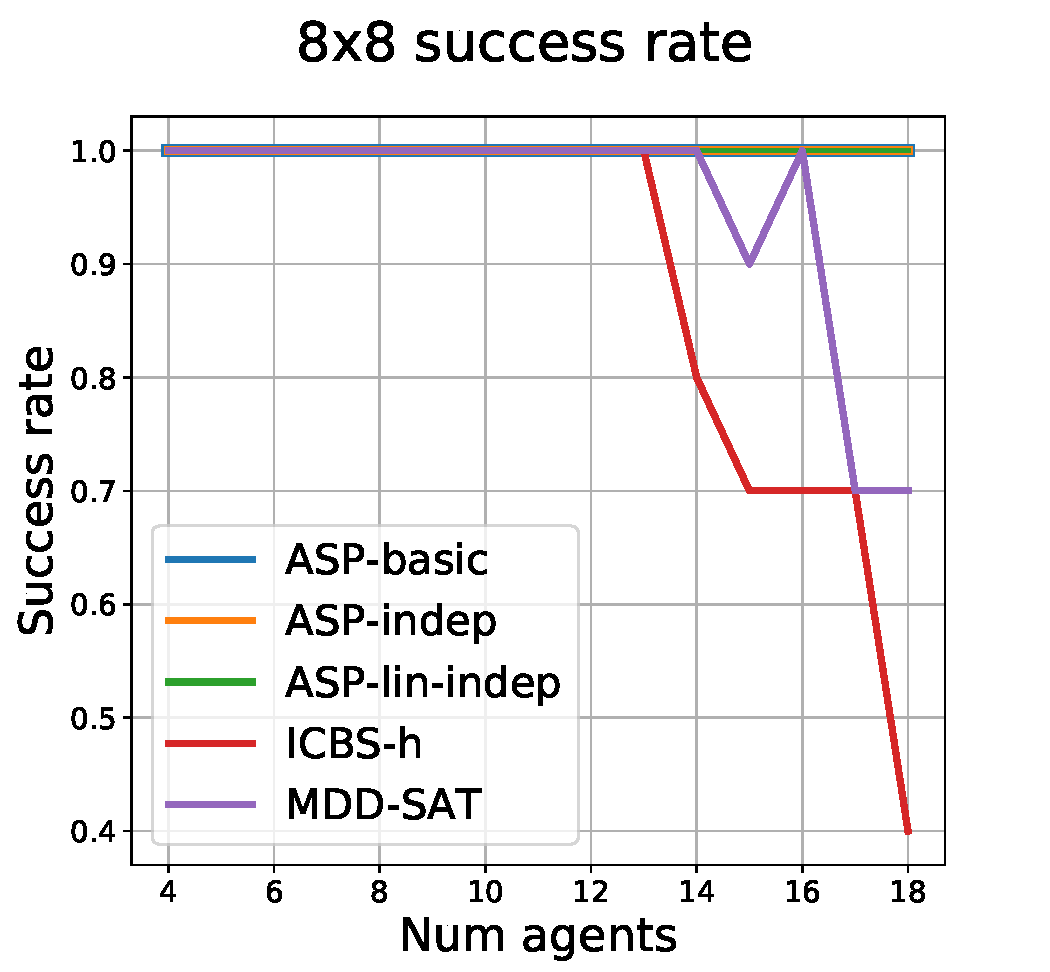
\includegraphics[width=0.24\textwidth]{graphs/8x8succ.pdf}
    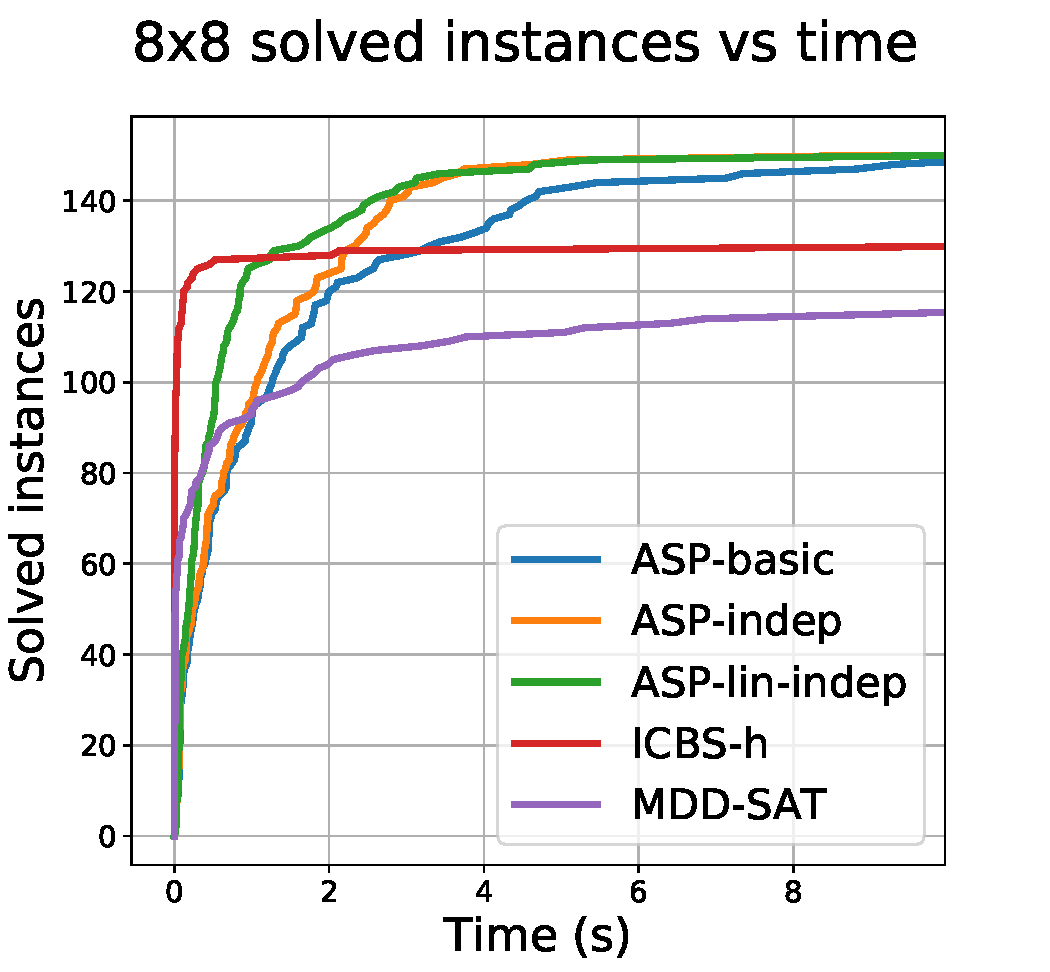
\includegraphics[width=0.24\textwidth]{graphs/8x8runtime.pdf}
    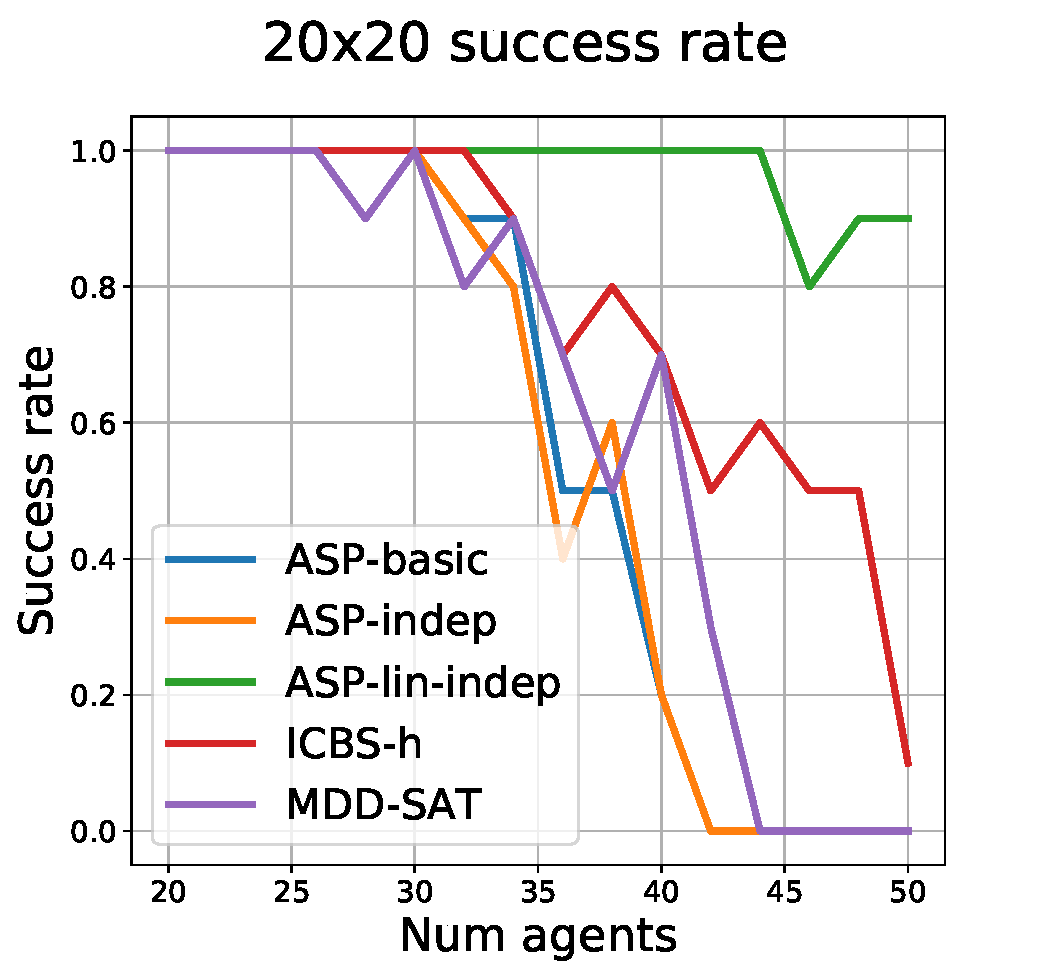
\includegraphics[width=0.24\textwidth]{graphs/20x20succ.pdf}
    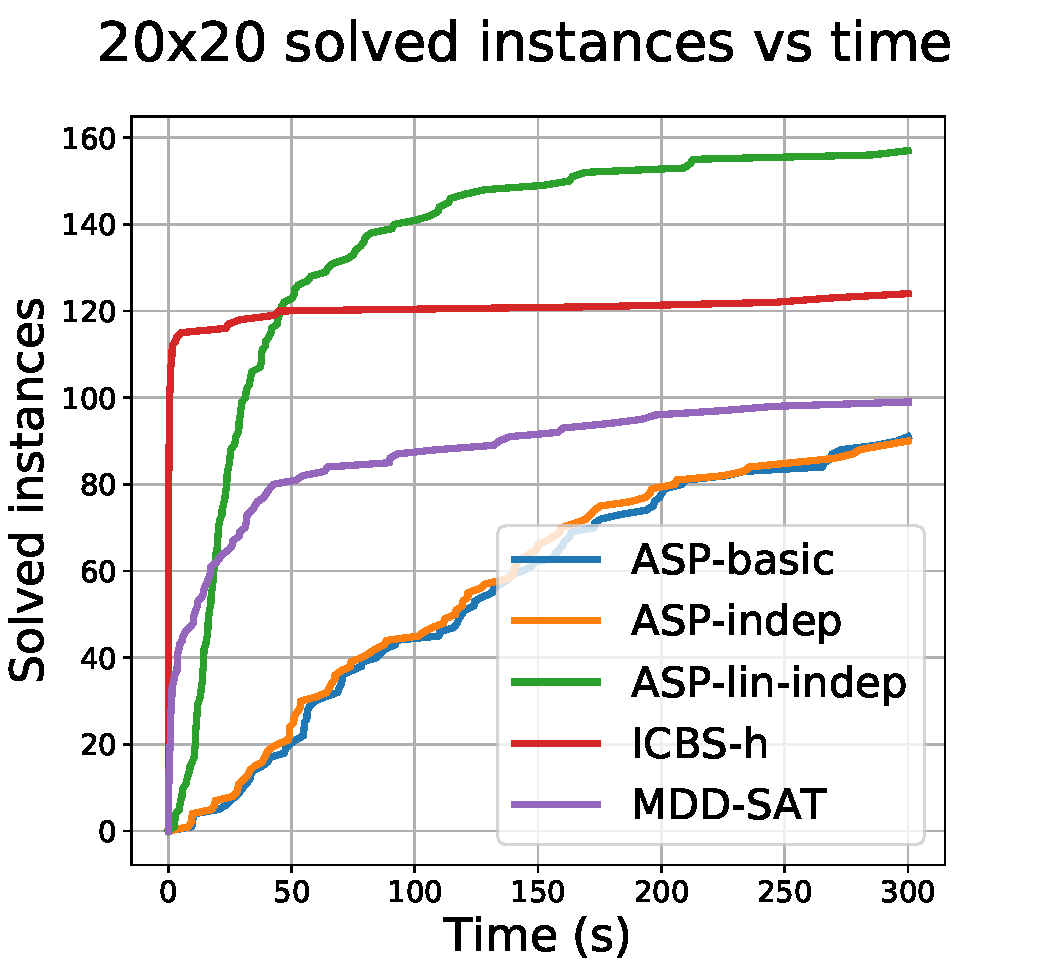
\includegraphics[width=0.24\textwidth]{graphs/20x20runtime.pdf}
    \caption{Success rate and number of instances solved versus time on $8\times 8$ and $20\times 20$ grids.}
    
    \label{fig_obs}
\end{figure*}

\begin{figure*}
    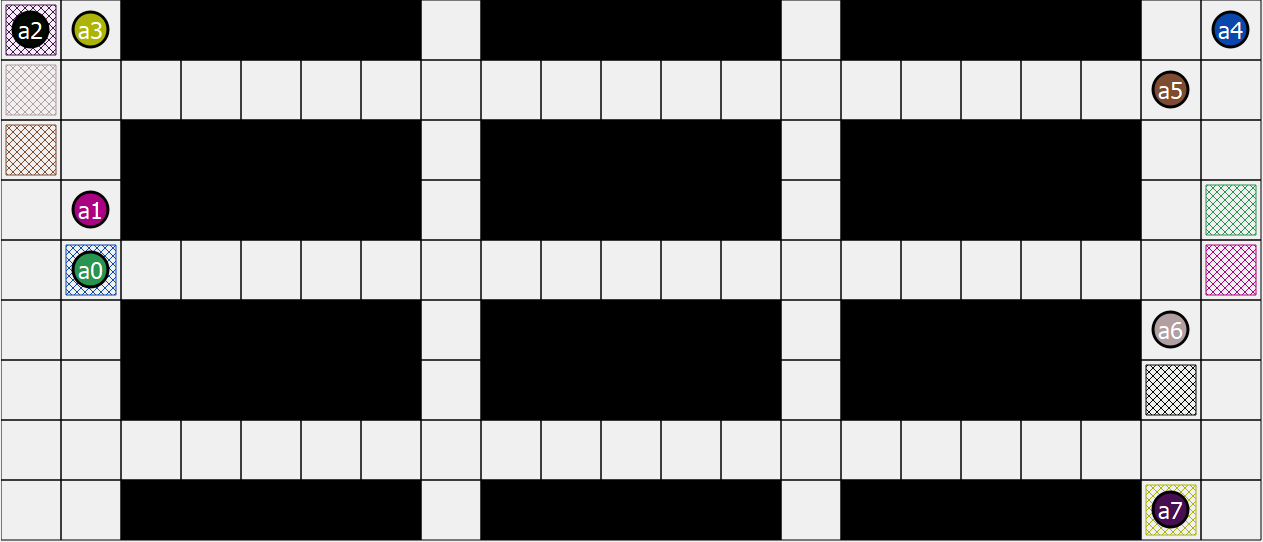
\includegraphics[width=0.45\textwidth]{graphs/warehouse.PNG}
    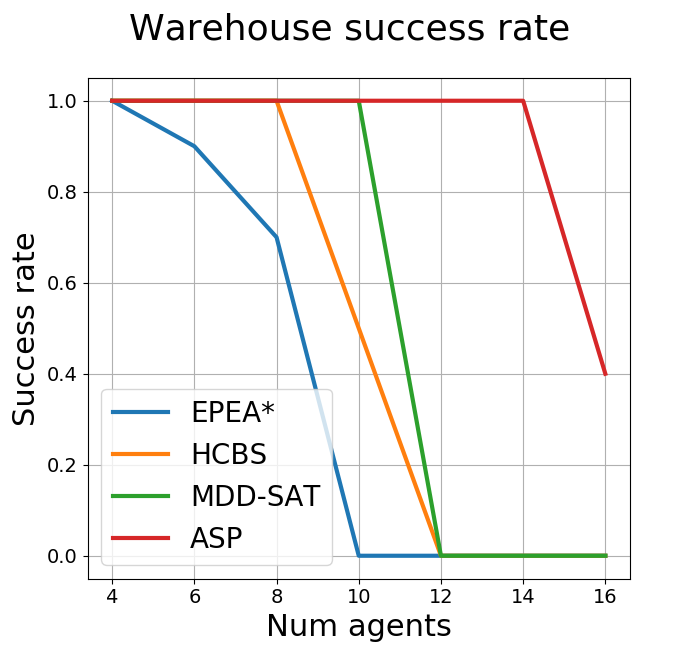
\includegraphics[width=0.24\textwidth]{graphs/warehousesucc.png}
    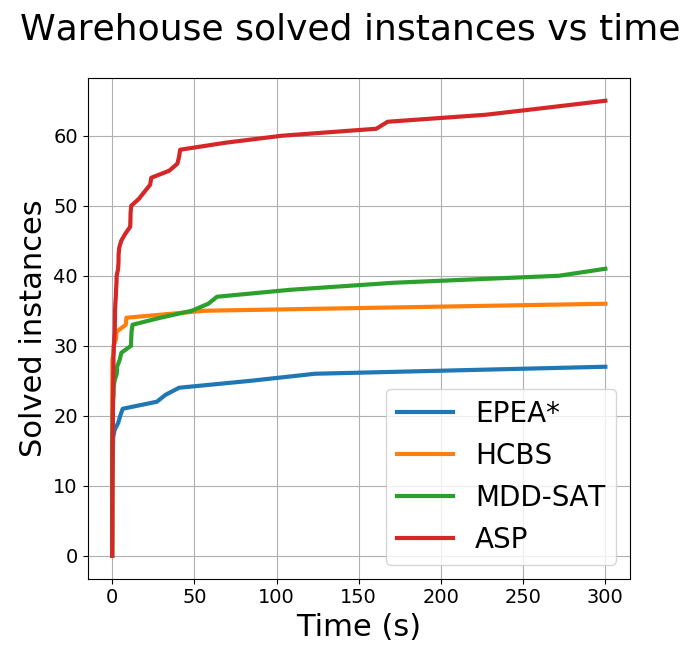
\includegraphics[width=0.24\textwidth]{graphs/warehouseruntime.png}
    \caption{Warehouse problem example and results}
    \label{fig_ware}
\end{figure*}

